\documentclass{article}

\usepackage[utf8]{inputenc}
\usepackage{listings}
\usepackage[margin=1in]{geometry}
\usepackage{graphicx, hyperref, mathpazo, units, breakurl}

\newcommand{\asm}[1]{\texttt{#1}}
\long\def\omitit#1{}

\title{\huge Lab 1: Introduction to Gumstix and Code Optimization}
\author{\Large\itshape 18--349 Embedded Real-Time Systems}
\date{
	Out: September 15, 2012, midnight EDT\\
	Due: September 29, 2012, midnight EDT \\
}

\begin{document}
	\maketitle

	\setcounter{tocdepth}{2}
	\tableofcontents
	\clearpage

	\begin{section}{Introduction to Part 1 of the Lab}
	\begin{subsection}{Overview} This part of the lab is meant to
	familiarize you with the hardware development platform and to
	introduce you to some good coding practices.  You will get acquainted with the hardware
	platform that we will be using throughout the course.  You
	will also learn to use a revision-control system.  You are
	strongly encouraged to continue using some form of revision-control
	system throughout the rest of the course.  Part 1 of this lab
	is meant to be neither difficult nor time consuming.  However, 
	this part of the lab is important, as the skills that it teaches
	will be a part of the assumed knowledge for future labs.  Of course, we also
	hope that it will be fun.  \end{subsection}

		\begin{subsection}{Tasks} In this part of Lab 1, you
		will perform a number of small tasks to get you warmed
		up and ready for further, more involved development in
		the class.  The embedded system in this class will be
		the gumstix verdex-pro+robostix system~\cite{gumstix:wiki}.  
		You will familiarize
		yourself with this system.  To this end, you will:
		\begin{enumerate} \item Create and use a source
		repository for your team~\ref{revision}.  \item Check
		out files from an SVN repository \emph{(15
		points)}~\ref{revision_task}.  
		\item Load the Linux kernel image and the root file system 
		to the microSD card \item Establish a
		serial connection from a provided gumstix embedded
		system to your computer~\ref{serial}.  \item Send it
		multiple files of different formats~\ref{files}.
		\item Boot a small GNU/Linux system on the
		gumstix~\ref{linux}.  \item Personalize the GNU/Linux
		system that you will use for the rest of the
		semester~\ref{mylinux}.  \item Program a simple Hello
		World program for the gumstix's ARM processor in C
		\emph{(20 points)}~\ref{helloworld}.  \item Program a
		simple program for the gumstix's ARM processor in ARM
		assembly \emph{(20 points)}~\ref{goodbyeworld}.  \item
		Disassemble and analyse binaries for the ARM \emph{(20
		points)}~ \ref{disassembly}.  \item Write a Makefile
		to automate the build process \emph{(20 points)}~
		\ref{makefile}.  \item Have fun!  \item Some points
		will be awarded for the proper compliance to instructions,
		the proper naming of files and the general quality of the handin.
		These are points to be assigned by the TAs at their discretion \emph{(5
		points)}.  \end{enumerate} \end{subsection}

		\begin{subsection}{Traditional Embedded Systems}
		Traditional embedded computers are low-power, low-memory devices.  Typically chosen to perform a
		specific task, embedded computers execute highly
		specialized software designed to function within the
		constraints of the devices.  In part due to these
		constraints, embedded systems software is almost
		always developed offline, often on a workstation that
		features a full software-development kit (SDK)
		including an editor, compiler, hardware simulator, and
		debugger.  \end{subsection}

		\begin{subsection}{Modern Embedded Systems} 
		% FIXME:exponential -- Verifiable claim?  
		% Priya look at this!  
		% Actual performance comparison between XScale and Pentium II/IIIs?  
		In the past few years, embedded
		computers have experienced an exponential growth in
		speed and memory capacity.  While many embedded
		systems still rely on traditional 8-bit
		microcontroller designs, embedded systems designed for
		communication or entertainment (cell phones, PDAs,
		handheld game consoles, etc.) feature 32-bit
		processors that can outperform desktop machines of ten
		years ago.  With flash memory offering persistent
		storage in the gigabyte range, it is now possible to
		natively develop embedded applications on the embedded
		systems themselves.  \end{subsection}

		\begin{subsection}{Embedded Systems for this Course}
			% Made some changes to allow for introduction of the simulator
			% if we want to.
			In this class, we will consider both the traditional and the on-system
			approaches of developing for embedded systems.  Some exercises will
			involve developing code offline while others will involve developing,
			compiling and testing code on the gumstix
			hardware itself.  In this lab, exercises will be carried out on the
			gumstix boards.  To successfully complete this lab, each group requires
			access to a computer with a USB port and software to perform terminal
			communication such as minicom or HyperTerminal.  All other hardware
			resources are provided to you by us in the form of a hardware kit.
		\end{subsection}
	\end{section}

	\begin{section}{Revision Control}
	\begin{subsection}{Introduction} A revision control or version
	control system is a toolset that assists programming teams in
	maintaining the history of and tracking changes made to a
	project that they are working on.  It is an essential tool for
	even two person teams when projects require multiple
	iterations of design and testing.  In this section, we shall
	describe the basic terminology related to a revision control
	system, how to set up a code repository, how to share work
	with your partners, how to track your partner's progress and
	how to work together, in parallel.  \end{subsection}

	\begin{subsection}{Basic Operations} All revision control
	systems have a concept of the `set of things it is in charge
	of'.  This set is usually a set of files or objects that the
	user has entrusted to the revision control system.  This set
	of files is called a \emph{repository} or a \emph{depot}.
	Revision control systems track all changes made in a
	repository by different users.  At regular intervals, the user
	commands the repository to take a snapshot of all the changes
	that have been made.  The tool now considers the repository to
	be at a new \emph{version} or \emph{revision}.  Changes such
	as what files have been added, what files have been removed,
	which lines have been changed and who changed them are all
	recorded.  This operation is known as a \emph{commit}.
	Suppose that a hardworking 18--349 group made a number of
	changes to their repository at 5 am.  The next day, they
	notice that they had mistakenly overwritten an important file.
	Thankful that they had used a revision control system, they
	ask the tool to undo all of the changes they had made.  This
	is known as a \emph{revert}.  Now consider two 18--349
	students who live off campus and work independently.  Instead
	of manually sending each other code, they each try to commit
	code to the repository that they have set up.  They notice
	that their changes overlap and that they need to cleverly
	adjust their edits to not overlap.  This operation of bringing
	together independent work on the same file is known as a
	\emph{merge}.  Any overlap in the code that is being merged
	causes a \emph{merge conflict} that must be manually
	\emph{resolved} by the merging user.  \end{subsection}

	\begin{subsection}{Client-Server Model} A client-server model
	of revision control is the traditional revision control model.
	The model consists of a primary server that hosts the
	repository or depot.  Users never directly edit the
	repository.  They \emph{check-out} a copy of the code out of
	the main repository.  They then edit their \emph{local} or
	\emph{working} copy to their hearts content.  When they are
	ready to show the world the work they have done, they commit
	their code.  But before they commit their code, they need to
	make sure that some one else hasn't changed the repository.
	Hence, they need to \emph{update} their working copy and
	resolve any merge conflicts.  They then commit their code to
	the main repository.  This model uses minimal space on client
	systems and has a canonical version history for the entire
	repository.  This model is used by traditional version control
	systems such as CVS~\cite{Grune:CVS},
	SVN~\cite{CollabNet:Subversion} and Perforce.
	\end{subsection}

	\begin{subsection}{Distributed Model} The upcoming models of
	revision control are all based on distributed, non-central
	models.  In these models, there is no one main repository.
	Each user's codebase is a bona fide repository in and of
	itself.  Users can \emph{clone} each others repositories to
	get each other's working copies.  Fundamental to this concept
	is the concept of \emph{branching} and independent histories.
	Since each user has their own independent repository, they
	each maintain their own version of the file histories.  The
	independent arcs of commits are known as \emph{branches}.  A
	branch in the repository signifies alternate histories of what
	happened to a repository.  Branches can be merged if they
	share a common version in the past known as an
	\emph{ancestor}.  Since multiple versions of a repository and
	its history are in flight at the same time, developers can
	easily choose which version they want to work on and who they
	want to merge with.  The tip of a branch that a developer is
	working on is known as the \emph{head} of that branch.  Since
	branching and merging are such common operations in a
	distributed model, special tools are used to deal with these.
	The most common is the three way merge used by
	Mercurial~\cite{Mackall:Mercurial} and
	Git~\cite{Torvalds:Git}.  A more advanced and formal system
	called patch calculus is used in Darcs~\cite{Roundy:Darcs}.
	\end{subsection}

	\begin{subsection}{Introduction to SVN} \label{revision} In
	this section, we shall introduce you to a popular revision
	control system called Subversion.  Subversion is a widely
	used, client-server model, multi-platform revision control
	system.  It is already installed on the ECE cluster machines
	and on all Andrew Unix machines.  Clients for it are available
	online~\cite{CollabNet:Subversion} including GUI versions for
	Windows XP and Vista.  We shall now go through a list of basic
	tasks and commands that you must get familiar with.  The tasks
	described can be performed on the ECE or Andrew Unix systems
	although they can be easily adapted to other environments as
	well.

	\begin{itemize} \item To create a new repository, use the
	\texttt{svnadmin} command.  
	\begin{verbatim} % svnadmin create /path/to/repository/here 
	\end{verbatim} 
	This directory will
	now act as the central storage area for all the code in your
	project.  Do not ever manually add, remove or modify files in
	this directory unless you want to seriously damage your
	repository.  Also note that the files that you work on in the
	project will not be stored in plain text in the main repo.  Do
	not go looking for them.

	\emph{Note: Due to an issue involving the bad interaction of
	AFS with the back-end of Subversion, file locking is flaky at
	best if Subversion is used on Andrew.  The course staff
	recommends that, should you choose to use subversion, that you
	host your repository on your own personal boxen or take
	regular snapshots of your Subversion repository should you
	choose to host it on Andrew.}

	\item To actually start creating and editing code, you will
	first need to get a \emph{working copy} of the (currently
	empty) repository.  This is the aforementioned
	\emph{check-out} operation.  
	\begin{verbatim} 
	% svn checkout file:///canonical/path/to/repository/here localcopy
	\end{verbatim} 
	The above command will create a working copy of
	the repository in the \texttt{localcopy} directory.  If you
	are checking out a file or project from a different machine
	than the repository, then use: 
	\begin{verbatim} 
	% svn checkout svn+ssh://username@server.ip.addr/path/to/repository/here  localcopy 
	\end{verbatim}

	\item You are now free to edit your code, add files and, in
	general, carry out your work in the \texttt{localcopy}
	directory.  For hints on how to organize your directory and a
	more thorough tutorial, consult this page by Sandler at Rice
	University~\cite{Sandler:SVNTutorial}.

	\item After you have done some work, it is now time to tell
	the repository to track the changes you have made.  Add the
	files to the tracker by issuing the following command.
	\begin{verbatim} 
	% svn add file1 file2 file3 
	\end{verbatim}

	\item To tell SVN to take a snapshot of your current progress
	as a \emph{revision}, issue the following command.
	\begin{verbatim} 
	% svn commit 
	\end{verbatim} 
	This command will bring up a text editor to allow you to properly and
	informatively label the changes you are going to commit.  The
	editor that it brings up depends on your \texttt{EDITOR}
	environment variable.  This variable is usually set in your
	\texttt{.bash\_profile}, \texttt{.cshrc} or equivalent file
	depending on your shell.  To find out what shell you are
	currently using, run: 
	\begin{verbatim} 
	% echo $SHELL
	\end{verbatim} 
	You can also temporarily change the
	\texttt{EDITOR} variable by using ``\texttt{export
	EDITOR=path/to/editor}" for bash or ``\texttt{setenv EDITOR
	path/to/editor}" for csh.

	\item You can now review your commits and changes using the
	\texttt{svn log} command.  You can also get elementary help by
	using the \texttt{svn help} command.

	\item The steps described above are extremely elementary.  Use
	this online SVN tutorial~\cite{RedBean:SVN} for a more
	complete description on how to import your teammate's code,
	how to merge changes and how to revert any mistakes that you
	may have made.  \end{itemize} \end{subsection}

	\begin{subsection}{Revision Control System Exercise (15 points)}\label{revision_task}
	
	We have created an SVN repository at
	\url{/afs/ece/class/ee349/jumpers} which you have read-access
	to.  Check out a working copy of this repository and then
	answer the following questions.  Record your answers in a
	plain text file called \texttt{repository.txt}.
	\begin{enumerate} \item Discounting hidden files, what are the
	files that are in the repository?  What are their names?  What
	are their contents?  \item What is the userid of the person
	(an ex-TA) who committed those files?  \item When did (s)he
	commit them (date and time) and what was the commit message?
	\end{enumerate} \end{subsection} \end{section}


	\begin{section}{Lab Hardware}
	\begin{subsection}{Hardware Kit Contents}
			
	Each lab group has been provided with a hardware kit with the
	following components:

	\begin{itemize}
		\item gumstix verdex-pro 400xm-bt motherboard
		\item gumstix robostix expansion board
		\item gumstix 5.0 volt power adapter
		\item Acroname USB serial interface connector
		\item Serial extension cable
		\item USB A--B cable
		\item \unit[2]{GB} microSD Card and Adapter
		%\item PXA--AVR UART jumper
	\end{itemize}

	\begin{figure}[t]
		\centering
		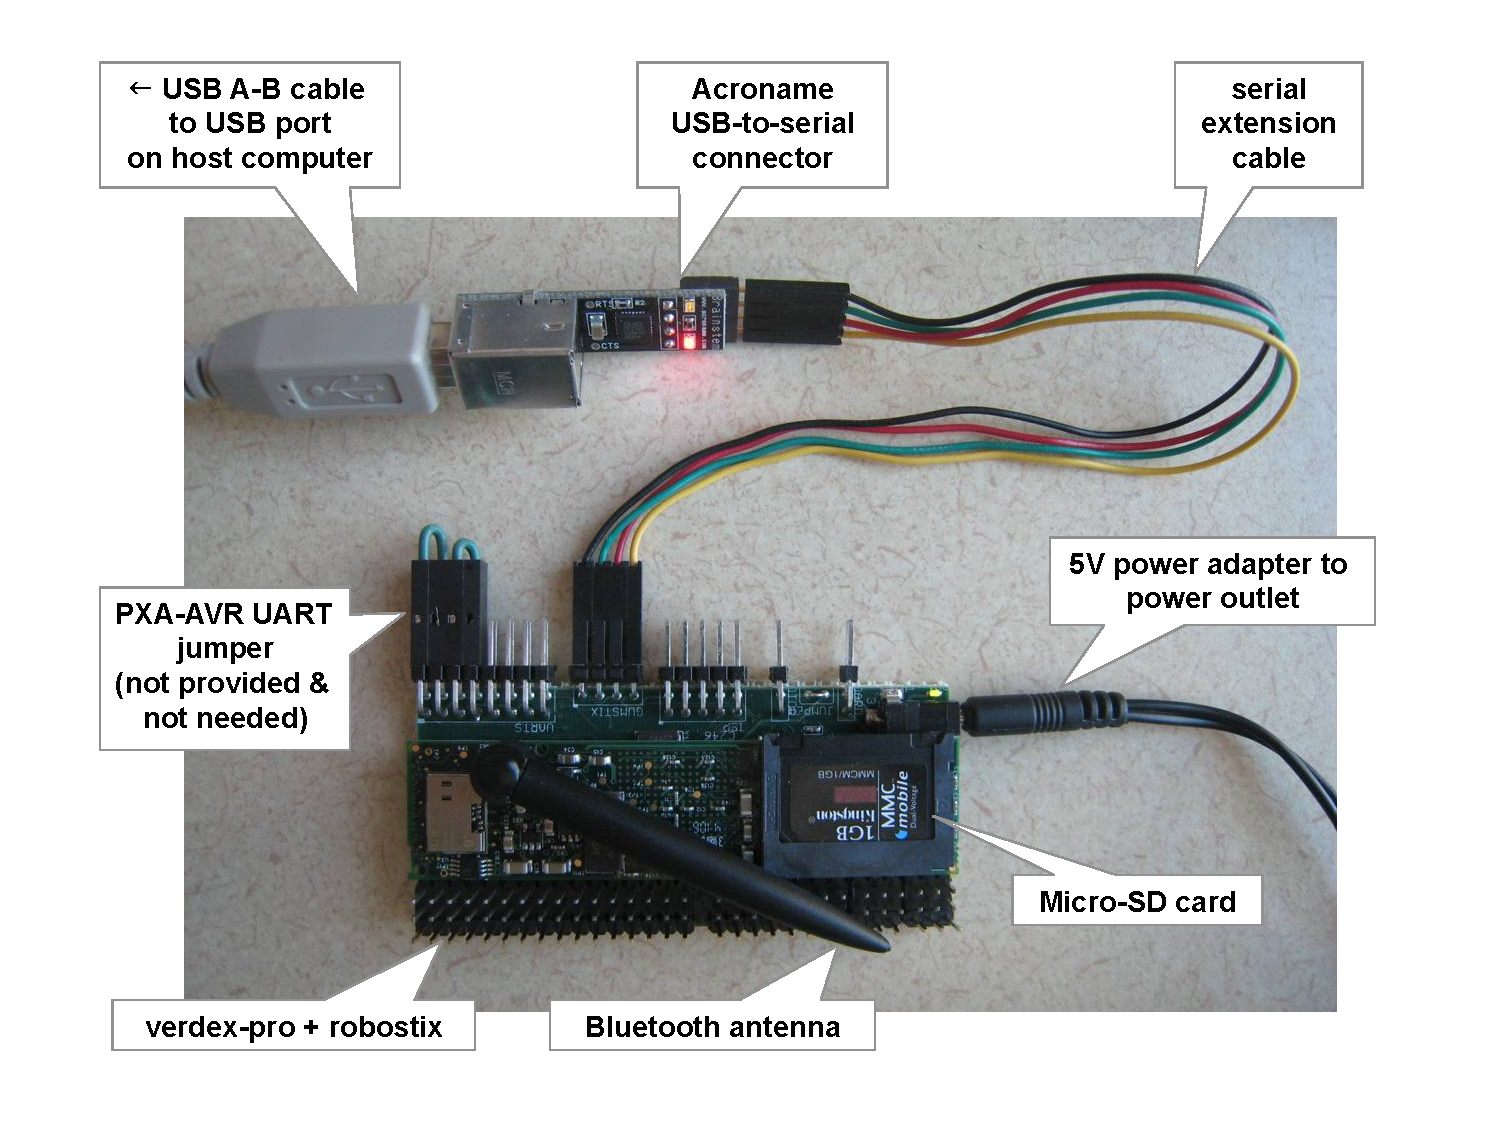
\includegraphics[width=\textwidth]{hardware-new}					\caption{Hardware kit components connected together.}
		\label{hardware}
	\end{figure}

	The heart of the 18--349 hardware kit consists of the verdex-pro
	motherboard and the robostix expansion board (see
	Figure~\ref{hardware}).  The verdex-pro motherboard is the smaller
	of the two boards and contains an Intel PXA270 processor(now
	owned by Marvel),
	\unit[16]{MB} of onboard flash memory, a miroSD card slot, and
	a Bluetooth module.  The robostix board is the larger of the
	two and contains an Atmel ATmega128 microcontroller with
	headers for nearly every I/O pin, as well as additional
	headers for some of the gumstix (PXA) I/O pins.

	The two boards may be connected by the white, 60-pin hirose
	connector.  When connected, the verdex motherboard sits
	in the center of channel of the robostix between the upper
	three rows of I/O headers and the power jack.  Since the
	verdex-pro motherboard itself lacks a power connector, it
	must always be used in conjunction with the robostix board to
	receive power.

	The third PCB is the USB serial interface connector.  It may
	connect to any of the gumstix (PXA) or robostix (AVR) UARTS,
	but is most often used to connect the Linux console on the
	gumstix to a host PC.  \end{subsection}

	\begin{subsection}{Hardware Setup} To setup the 18--349
	hardware: 
	\begin{enumerate} 
	\item Insert the microSD into the card slot on the motherboard.

	\item Gently snap the verdex motherboard into the
	robostix so that the motherboard lies entirely on top of the
	robostix (as opposed to hanging off the other side).

	\item Ignore the PXA--AVR UART jumper shown in Figure ~1. This is not provided in your hardware kit, and you will not need the jumper for the labs (the jumper is shown purely for the sake of completeness because it might be required for interaction between the verdex-pro and the robostix for hobby projects and other extensions).

	\item Connect the male side of the four wire
	(black/green/red/yellow) extension cable to the ``Brainstem''
	port of the serial converter.  The black wire should connect
	on the left side when the converter is oriented such that the
	word ``Brainstem'' reads properly (i.e., Brainstem port on
	top, USB port on bottom).

	\item Connect the female side of the four wire extension cable
	to the ``GUMSTIX'' pins on the robostix board.  The black wire
	should connect on the right side when the robostix board is
	oriented such that the word ``GUMSTIX'' reads properly (the
	pins are on the bottom).

	\item Connect the USB A-B cable first to the serial converter,
	then to a USB port on the host computer.  If the host computer
	is running Windows XP, Windows Vista or Mac OS, you may need
	to install the latest FTDI Virtual COM Port
	Driver~\cite{FTDI:VCP} before or while completing this step.
	The FTDI driver should already be available on most Linux
	machines.  \end{enumerate} % 
	Note: Do \emph{not} connect the
	gumstix power adapter until after setting up serial
	communications on the host machine as described in the next
	section.  \end{subsection} \end{section}

	\begin{section}{Communicating with the Gumstix} \label{serial}
	\begin{subsection}{RS--232 Serial Communications}
	
	The principal means of communicating with the gumstix boards
	is through an RS--232 serial connection.  RS--232 is a nearly
	forty-year old standard for serial data signals between
	computers and peripheral equipment such as terminals, modems,
	printers, and mice.  Until a few years ago RS--232 serial
	ports were found on nearly every desktop \& workstation
	computers.  Since then, the rising popularity of RS--232's
	successor protocol, the Universal Serial Bus (USB), has seen
	the elimination of RS--232 ports (along with other legacy I/O)
	ports from consumer machines.  However, due to the simplicity
	\& robustness of the protocol, RS--232 is still heavily
	featured in both embedded and enterprise systems.

	In the context of the gumstix, RS--232 is used to communicate
	with the gumstix U-Boot bootloader and Linux console, much as
	a keyboard and monitor is used to communicate with a Linux
	desktop machine.  A Universal Asynchronous
	Receiver/Transmitter (UART) serves as a ``serial controller,''
	and is used by software programs to convert parallel data
	(typically bytes) to serial signals and back.

	The gumstix PXA processor contains four UARTs, two of which
	are accessible via four-pin headers on the robostix board.
	The first accessible UART (FFUART) is typically controlled by
	the Linux console.  The second accessible UART (STUART) is
	available for general purpose use, including its use in
	programming the AVR microcontroller.  The AVR itself also
	features two UARTS.  The USB serial interface connector also
	contains a UART which is accessible over USB by a host
	computer.  
	\end{subsection}

	\begin{subsection}{Host Communications Setup} \label{hostcomm}
			
	To communicate with the gumstix console, the host PC must run
	terminal communication software such as minicom or
	HyperTerminal.  Terminal communication software was once
	popularly used in conjunction with modems for text-mode access
	to computer Bulletin Board Systems (BBSes) and remote Unix
	systems.\footnote{With the rise in popularity of the Internet,
	text-mode terminal connections were replaced by SLIP and PPP
	to enable the connecting machine to participate in the IP
	network directly---this is what's now known as ``dialup
	Internet.''}  Connecting to the gumstix with terminal software
	is exactly like connecting to a remote Unix system, except
	that there's no modems or phone lines involved.

	To communicate with the gumstix, the terminal software must be
	configured to use the USB serial device at \unit[115200]{bps}
	with 8 data bits, no parity, 1 stop bit, and no flow control
	(neither hardware (RTS/CTS) nor software (XON/XOFF)).  The
	following sections provide step-by-step guides for configuring
	these settings in popular terminal software packages.

	\begin{subsubsection}{Configuring Minicom on Linux} To
	configure minicom for connecting to the gumstix console on
	Linux:\\\\
    (NOTE: In some versions of Linux, all ``\verb|minicom|''
	commands must be run with ``\verb|sudo|'' in front of them
	(``\verb|sudo minicom -sc on|'', for example). Your mileage may vary.):

	\begin{enumerate} 
		\item Execute ``\verb|minicom -sc on|'' to bring up the configuration menu.

		\begin{item}
						Make the following changes under the ``Serial port setup'' menu:
						%
						\begin{itemize}
							\item Change ``Serial Device'' to ``/dev/ttyUSB0''\footnote{Or the
							      appropriate device if not ttyUSB0.}
							\item Change ``Bps/Par/Bits'' to 115200 8N1.
							\item Change ``Hardware Flow Control'' to ``No''.
							\item Change ``Software Flow Control'' to ``No''.
						\end{itemize}
					\end{item}

					\begin{item}
						Make the following changes under the ``Modem and dialing'' menu:
						%
						\begin{itemize}
							\item Clear the ``Init string'' field.
							\item Clear the ``Reset string'' field.
							\item Clear the ``Hang-up string'' field.
						\end{itemize}
					\end{item}

					\item Select "Save setup as dfl".
					\item Select "Exit from Minicom".
				\end{enumerate}
				%
				To invoke minicom for normal operation:
				%
				\begin{itemize}
					\item Execute ``\verb|minicom -c on|'' to enter minicom.
					\item Type ``\verb|C-A q|''\footnote{``\texttt{C-A}'' means ``press \& hold
					      the \texttt{control} key while pressing the \texttt{a} key.''} to exit
					      minicom.
				\end{itemize}
			\end{subsubsection}

			\begin{subsubsection}{Configuring HyperTerminal on Windows XP} \label{hyperterm_xp}
				To configure HyperTerminal for connecting to the gumstix console on Windows
				XP:
				%
				\begin{enumerate}
					\item Execute HyperTerminal from the Start menu (located in Accessories,
					      Communications).
					\item Cancel the ``Location Information'' dialog every time it appears.
					\item Enter ``gumstix'' for the connection name, click OK.
					\item Select the highest COM port under ``Connect using'',\footnote{Or the
					      appropriate device if not the highest COM port.} click OK.

					\begin{item}
						Select these settings on the ``COM Properties'' dialog:
						%
						\begin{center}
							\begin{tabular}{|ll|}
								\hline %--------------------
								Bits per second: & 115200 \\
								Data bits:       & 8      \\
								Parity:          & None   \\
								Stop bits:       & 1      \\
								Flow control:    & None   \\
								\hline %--------------------
							\end{tabular}
						\end{center}
					\end{item}

					\item Exit HyperTerminal, save the connection settings.
				\end{enumerate}
				%
				To invoke HyperTerminal for normal operation, execute HyperTerminal via
				\texttt{gumstix.ht} from the Start menu (located in Accessories,
				Communications, HyperTerminal).
			\end{subsubsection}

			\begin{subsection}{Configuring HyperTerminal on Windows Vista}
				Hyperterminal is not available in Windows Vista by default.  You can
				acquire Hyperterminal by copying the executable and dlls from a Windows
				XP machine.  For your convenience, the relevant files are compressed
				and placed on the course web site. Simply extract the
				contents of the archive and double click on \texttt{hyperterm.exe} to
				run Hyperterminal.

				When you first connect the brainstem to your Windows Vista machine, a
				pop-up bubble should notify you of the COM port alloted to the brainstem.
				Use this COM port when configuring Hyperterminal.  You can now use the
				instructions in section \ref{hyperterm_xp} to configure your Hyperterminal.

				If you are having problems connecting with HyperTerminal, it may be
				because Windows has not have configured the brainstem correctly.  Go to the
				Windows ``Device Manager", right-click and select the properties option for the
				COM port.  Check that the Baud rate/Data bit/Parity/Stop bit/flow control etc.
				are as stated in Section \ref{hostcomm}.
			\end{subsection}
		\end{subsection}

		\begin{subsection}{Transferring Files} \label{files}
			An RS--232 serial connection, much like Ethernet, is inherently unreliable.
			Thus, weak serial transmissions occasionally garble or even drop
			characters.  While corruption is rare enough that it usually does not
			hinder one's ability to read text, corruption is deleterious to
			transferring binary data.

			Much as TCP was designed to provide reliable communication streams in
			unreliable network environments, numerous file transfer
			protocols\footnote{Kermit \& ZMODEM are the two most popular protocols.
			XMODEM \& YMODEM were once popular but are now deprecated.} have been
			developed to enable reliable file transfers over serial connections.  For
			transferring files with the gumstix, we recommend using the ZMODEM
			protocol as it is both fast and easy to use.

			\begin{subsubsection}{Transferring Files via ZMODEM in Minicom}
				To upload a single file from the host PC to the gumstix:
				%
				\begin{enumerate}
					\item Make sure the gumstix console is sitting at a shell prompt.  The
					      \texttt{lrz} program will be invoked automatically by minicom.
					\item Type ``\verb|C-A s|'' to bring up the ``Upload'' menu and select
					      ``zmodem''.
					\item Navigate to the appropriate location, pressing \texttt{SPACE} twice
					      to enter a directory.
					\item Tag the appropriate file by pressing \texttt{SPACE} once, then press
					      \texttt{ENTER} to begin the transfer.
				\end{enumerate}
				%
				To download a single file from the gumstix to the host PC:
				%
				\begin{enumerate}
					\item Execute ``\verb|lsz -b filename|'' to initiate a ZMODEM transfer for
					      the file ``filename''.
					\item Minicom will automatically start downloading the file.
				\end{enumerate}
			\end{subsubsection}

			\begin{subsubsection}{Transferring Files via ZMODEM in HyperTerminal}
				To upload a single file from the host PC to the gumstix:
				%
				\begin{enumerate}
					\item Make sure the gumstix console is sitting at a shell prompt.  The
					      \texttt{rz} program will be invoked automatically by HyperTerminal.
					\item Select ``Send File'' from the ``Transfer'' menu.
					\item Select the appropriate file to upload, choose ``Zmodem with Crash
					      Recovery'' under ``Protocol'', click Send.
				\end{enumerate}
				%
				To download a single file from the gumstix to the host PC:
				%
				\begin{enumerate}
					\item Execute ``\verb|sz -b filename|'' to initiate a ZMODEM transfer for
					      the file ``filename''.
					\item HyperTerminal will automatically start downloading the file.
				\end{enumerate}
			\end{subsubsection}

			\begin{subsubsection}{Transferring Multiple Files}
				Minicom and \texttt{sz} both allow multiple files to be transmitted via
				ZMODEM in the same invocation.  However, since the serial link is slow and
				ZMODEM uses no compression internally, transferring many files may be a
				time consuming process.

				An alternative for transferring multiple files is to create a compressed
				archive of the directories or files desired to transmit and transmit the
				compressed archive instead (see Section~\ref{tar} for details on using tar
				to create compressed archives).
			\end{subsubsection}
		\end{subsection}
	\end{section}
	
	\begin{section} {Preparing Your Gumstix} \label{prepare}
	Before you can start working on the Gumstix, you need to load
	the microSD card with a boot script, a kernel image and a root
	file system. The boot script, kernel image and the file system
	are available from the course website at
	\url{http://www.ece.cmu.edu/~ee349/projects.html}. Before you
	can load the card, you will have to create two partitions on
	the card. The instructions for partitioning the microSD card,
	loading the kernel image and loading the file system are provided
	in the document
	\url{http://www.ece.cmu.edu/~ee349/docs/verdex-setup.pdf} . If
	you face any difficulty in this process, you should contact the 
	course staff immediately.
	\end{section}
	

\begin{section}{Gumstix Programming Environment} \label{linux}
		\begin{subsection}{Introducing the Gumstix}
			Once the gumstix hardware is setup and terminal communication software is
			setup and running on the host, connect the gumstix power adapter to power
			on and boot the gumstix.

			When the gumstix boots, the first text that appears on the serial console
			reads:
			%
			\begin{verbatim}
				U-Boot 1.2.0 (May  10 2008 - 21:17:19) - PXA270\@400 MHz - 1604

				*** Welcome to Gumstix ***

			
				DRAM :  64 MB
				Flash: 16 MB
				Using default environment

			\end{verbatim}
			%
			U-Boot~\cite{DENX:U-Boot} is the gumstix bootloader.  It is a very popular
			bootloader used in many 32-bit embedded systems, and is responsible for the
			initial hardware setup before passing control to the kernel.  U-Boot will
			also be one of the target environments for programming in later labs.

			As U-Boot proceeds, it detects a file system and Linux kernel on the microSD cards.
			U-Boot loads the kernel into memory, then transfers control to the Linux
			kernel itself.  The Linux kernel initializes the remaining peripheral
			hardware and launches the userspace \texttt{init} process.  Eventually when
			userspace initialization is complete, you're greeted with the login prompt
			on the serial console:
			%
			\begin{verbatim}
			Welcome to the Gumstix Linux Distribution!

			gumstix login:
			\end{verbatim}
			%
			Let's login:
			\begin{enumerate}
				\item Enter ``\texttt{root}'' as the login name.
				\item Enter ``\texttt{gumstix}'' as the password.
			\end{enumerate}
			%
			This will bring you to a Bash shell prompt:
			%
			\begin{verbatim}
			Welcome to the Gumstix Linux Distribution!

			gumstix login: root
			Password:
			Welcome to Gumstix!
			[root@gumstix ~]#
			\end{verbatim}
			%
			In the following sections, the (``\verb|#|'') prompt indicates commands
			that should be typed, and the non-``\verb|#|'' statements that follow
			indicate program output (or logical equivalent) that will be displayed as
			result.
		\end{subsection}

		\begin{subsection}{Personalizing the Gumstix} \label{mylinux}
			After logging in, the first thing we ask you and your lab group
			to do is to personalize your board.  At minimum, you should give your board
			a unique hostname (so that it is easily discernible in a Bluetooth scan),
			and a unique root password (so nobody can login).  Follow these commands to
			set both:
			%
			\begin{verbatim}
				# echo "choose_a_new_hostname" > /etc/hostname
				# busybox hostname -F /etc/hostname
				# passwd
				Changing password for root
				Enter the new password (minimum of 5, maximum of 8 characters)
				Please use a combination of upper and lower case letters and numbers.
				Enter new password:
				Re-enter new password:
				Password changed.
			\end{verbatim}
		\end{subsection}

		\begin{subsection}{Shell \& Environment}
			When you login to the gumstix as root, the shell starts with a working
			directory of \texttt{/root}.\footnote{This may be verified by executing
			``\texttt{pwd}''.}  We recommend that all work performed on the gumstix be
			located in \texttt{/root} or a subdirectory thereof.

			Installed on the microSD rootfs is the full set of GNU Coreutils (\texttt{cat},
			\texttt{cp}, \texttt{echo}, \texttt{ln}, \texttt{mkdir}, \texttt{mv},
			\texttt{pwd}, \texttt{rm}, \texttt{rmdir}, etc.)~\cite{FSF:GNUCoreutils}
			and other GNU utilities (\texttt{find}, \texttt{grep}, etc.).  Although we
			do not expect you to be an expert, you should have some familiarity with
			the these tools as they will be essential for working in the gumstix
			environment.  If you are unfamiliar with them, please consider trying a
			GNU/Linux tutorial.

			To reboot the gumstix, execute the command ``\verb|reboot|''.  To halt or
			power off the gumstix, execute:
			%
			\begin{verbatim}
			# halt
			...
			The system is going down NOW !!
			Sending SIGTERM to all processes.
			The system is halted.
			System halted.
			\end{verbatim}
			%
			Once the gumstix reports ``\verb|System halted.|'' it is safe to power off
			the gumstix.  If you need to hard reboot the gumstix, simply power off the
			gumstix normally, then power it back on.\footnote{There is a reset switch
			on the underside of the verdex-pro board.  However, it is extremely
			inconveniently placed when connected to the robostix.  Don't waste your
			time with it.}
		\end{subsection}

		\begin{subsection}{Tar \& Compressed Archives}\label{tar}
			Tar~\cite{FSF:GNUTar} is the traditional Unix utility for creating file
			archives.  In the context of the gumstix platform, compressed file archives
			are useful for transferring multiple files over a slow serial connection.

			Tar is typically used to compress a directory including all files and
			subdirectories within.  Since the archives produced by tar are
			uncompressed, various file compression utilities are often used in tandem
			with tar.  These compression utilities typically can only compress and
			decompress a single file, hence the need to pair them with an archiver.
			The combined output of the archiver and compressor is a compressed archive
			somewhat analogous to the popular ZIP archive format.

			While tar itself is nearly ubiquitous\footnote{An occasionally used
			alternative is cpio.}, each of the various compression
			utilities\footnote{Includes gzip, bzip2, lzop, lzma, compress, and others.}
			have various benefits and tradeoffs in terms of compression ratio, speed,
			complexity, and patent restrictions.\footnote{See LZW algorithm \& Unisys
			patent debacle.}  The most popular Unix compressor is
			gzip~\cite{Gailly:gzip}, which offers median performance in terms of both
			compression ratio and encoding/decoding speed.\footnote{Uses the same
			DEFLATE compression algorithm as the ZIP format.}

			To create a tar\,+\,gzip (.tar.gz) compressed archive of the example
			directory \texttt{foo} and all its contents, execute the commands:
			%
			\begin{verbatim}
				# tar cvf foo.tar foo
				(list of files added to archive)
				...
				(creates foo.tar)
				# gzip -9 foo.tar
				(creates foo.tar.gz)
			\end{verbatim}
			%
			Due to gzip's popularity as a compressor for tar archives, many versions of
			tar include an option to call gzip internally, allowing the entire
			compressed archive to be created in one command:
			%
			\begin{verbatim}
			# tar cvzf foo.tar.gz foo
			\end{verbatim}
			%
			The now completed .tar.gz archive may be transferred to the host PC over
			ZMODEM.

			When ZMODEM is used to send a .tar.gz archive from the host PC, the
			original directory structure may be extracted from the archive with the
			command:
			%
			\begin{verbatim}
			# tar xvzf foo.tar.gz
			(creates directory foo/ and lists files extracted)
			...
			\end{verbatim}
		\end{subsection}

		\omitit{
		\begin{subsection}{Coding \& Editors}
			The course staff recommends that most of your group's coding be done on a
			host machine and not on the gumstix itself.  Due to the fragile nature of
			the microSD cards, any significant code changes made on the microSD cards 
            could be lost before you have a chance to transfer and backup.

			Given the nature of the typical ``edit, compile, debug'' cycle, it is
			practical to make minor code changes on the gumstix itself while debugging.
			However, be sure not to leave any code on the microSD that can't be
			rewritten or remodified in case of loss.

			For when you do need to edit code on the gumstix, there are three editors
			installed on the microSD rootfs: GNU nano, JED, and Vim.  Here is a brief
			description of each:

			\begin{paragraph}{GNU nano.}
				nano~\cite{NCDT:GNUnano} is a clone of Pico (of Pine fame) and is the
				simplest of the three editors.  nano's feature set is, however, limited in
				comparison to the other two.  To use nano, execute
				``\verb|nano|''.\footnote{If the screen appears garbled, try executing
				``\texttt{TERM=vt100}'' first.}
			\end{paragraph}

			\begin{paragraph}{JED.}
				JED~\cite{Davis:JED} is a powerful but friendly programmer's editor.  JED
				emulates Emacs by default, and is a reasonable choice for those familiar
				with Emacs.\footnote{Emacs itself could not be included due to its size and
				consistent refusal to cross compile.}  To use JED, execute ``\verb|jed|''.
			\end{paragraph}

			\begin{paragraph}{Vim.}
				Vim~\cite{Moolenaar:Vim} is a very powerful vi-like editor.  Although quite
				popular with Unix programmers, it is often regarded as unintuitive and as
				having a steep learning curve.  Unless you're already proficient in Vim or
				want to commit to learning it, it's probably best to avoid in favor of JED.
				To use Vim, execute ``\verb|vim|''.\footnote{If you didn't follow the
				advice given, and are now stuck in Vim, type ``\texttt{:q!}'' to quit.}
			\end{paragraph}
		\end{subsection}
		}

		\begin{subsection}{Compilers \& Development}
			Traditionally, code for an embedded system is compiled on a desktop or
			workstation computer with a cross compiler.\footnote{A cross compiler
			generates code for a target platform that is different from the host
			platform on which the compiler executes.}  To maximize lab consistency and
			to minimize the software requirements of the host PC, 18--349 labs will
			actually be compiled on the gumstix hardware itself.

			The microSD rootfs features two compilers, a GCC ARM native compiler
			(\texttt{gcc})~\cite{FSF:GCC}, and a GCC AVR cross compiler
			(\texttt{avr-gcc}).  In addition, the microSD rootfs contains both AVR
			Libc~\cite{Roth:AVRLibc}, and (ARM Linux) uClibc~\cite{Andersen:uClibc}, as
			well as other traditional Unix development tools such as diff/patch and GNU
			make.
		\end{subsection}
	\end{section}

	\begin{section}{Gumstix Programming Exercises}
		The following programming exercises are meant to serve as a tutorial
		introduction to writing, compiling, executing, and debugging code on the
		ARM platform.  While the code is simple, the procedural exercise will be
		invaluable in preparing for later labs.

		\begin{subsection}{Hello World on ARM (20 points)} \label{helloworld}
			Complete these steps to write a ``Hello world!'' application on ARM:
			%
			\begin{enumerate}
				\item Boot the gumstix and login as \texttt{root}.

				\begin{item}
					Create a \texttt{/root/lab0/hello} project directory:
					%
					\begin{verbatim}
						# mkdir -p ~/lab0/hello
						# cd ~/lab0/hello
					\end{verbatim}
				\end{item}

				\item Using the editor of your choice, edit the file \texttt{hello.c}.

				\begin{item}
					In \texttt{hello.c}, write a version of the canonical ``Hello world!''
					program that:
					%
					\begin{itemize}
						\item Writes the string ``\texttt{Hello world!}'' followed by a new line to
						      \emph{stdout}.
						\item Terminates with exit status 0.
						\item Style and comment your code properly.
					\end{itemize}
				\end{item}

				\begin{item}
					Compile \texttt{hello.c} by executing the commands below, and verify that
					your output is proper:
					%
					\begin{verbatim}
						# gcc -Wall -Werror -o hello hello.c
						# ./hello
						Hello world!
					\end{verbatim}
				\end{item}
			\end{enumerate}
		\end{subsection}

		\begin{subsection}{Goodbye World on ARM (20 points)} \label{goodbyeworld}
			Complete these steps to write a ``Goodbye world!'' application on ARM:
			%
			\begin{enumerate}
				\begin{item}
					Generate the assembly code for the \texttt{hello.c} program:
					%
					\begin{verbatim}
						# gcc -S -Wall -Werror hello.c
						(creates hello.s)
					\end{verbatim}
				\end{item}

				\item Create a new \texttt{/root/lab0/goodbye} project directory.

				\item Copy the \texttt{hello.s} assembly code to the new project directory
				      and rename it \texttt{goodbye.s}.

				\begin{item}
					Modify \texttt{goodbye.s} assembly code so that the new behavior of the
					program is:
					%
					\begin{itemize}
						\item Writes the string ``\texttt{Hello world!}'' followed by a new line to
						      \emph{stdout}.
						\item Writes the string ``\texttt{Goodbye world!}'' followed by a new line
						      to \emph{stdout}.
						\item Terminates with exit status 42.
						\item Comment your code properly.
					\end{itemize}
				\end{item}

				\begin{item}
					Assemble \texttt{goodbye.s} by executing the commands below, and verify
					that your output matches:
					%
					\begin{verbatim}
						# gcc -o goodbye goodbye.s
						# ./goodbye
						Hello world!
						Goodbye world!
					\end{verbatim}
				\end{item}
			\end{enumerate}
		\end{subsection}

		\begin{subsection}{Disassembly (20 points)}\label{disassembly}
			Complete the following steps to disassemble the ``Hello world!'' application:
			%
			\begin{enumerate}
				\item Change back to the \texttt{/root/lab0/hello} project directory.

				\begin{item}
					Disassemble the \texttt{hello} executable with the following commands:
					%
					\begin{verbatim}
						# objdump -d hello > hello-d.txt
						# objdump -D hello > hello-D.txt
					\end{verbatim}
				\end{item}

				\item Transfer \texttt{hello-d.txt} \& \texttt{hello-D.txt} to the host
				      machine and analyze them.
			\end{enumerate}
			%
			Each question is worth five points.
			Record your answers to the following questions in a plain text file
			called \texttt{disassembly.txt}:
			%
			\begin{enumerate}
				\item What is the entry point address of the program?  (Hint: The
				      \texttt{readelf} program may provide a clue.)

				\item What is the name of the first function branched to in the program?
				      (Hint: One of \verb|readelf -s|, \verb|readelf -r|,
				      \verb|objdump -t|, or \verb|objdump -T| may provide a clue.)

				\item What is the \emph{key} difference between the output of \verb|objdump -d|
				      (\texttt{hello-d.txt}) and \verb|objdump -D| (\texttt{hello-D.txt})?

				\item Is the interpretation of the instructions under the \texttt{.rodata}
				      section of \texttt{hello-D.txt} correct?  What does this
				      interpretation mean?
			\end{enumerate}
		\end{subsection}
	\end{section}

	\begin{section}{Automating the Build Process with Make (20 points)}\label{makefile}
		Manually rebuilding executables as part of the ``edit, compile, debug''
		cycle quickly becomes a time consuming and tedious task, especially for
		large projects with many source files.  The traditional Unix development
		utility used to automate and manage the build process is
		Make~\cite{FSF:GNUMake}.

		Projects using Make ship with a \texttt{Makefile} which describes how to
		build various ``targets'' of the project from source files.  When Make is
		invoked as ``\texttt{make}'', it builds the first target listed in the
		Makefile, which is typically the project executable in its default
		configuration.  Most projects contain other useful targets such as
		``\texttt{make clean}'' which typically removes all temporary object files
		used in the building process.

		\begin{subsection}{Makefiles at a Glance}
			A \texttt{Makefile} is a plain text file that contains a set of rules.
			Each rule describes how to generate a target file from a list of
			prerequisite files and a list of shell commands.  Makefile rules have the
			form:\footnote{Commands specified in a rule \emph{must} be indented by a
			tab, and not spaces.}
			%
			\begin{verbatim}
			target: prerequisites ...
			        commands to build target from prerequisites
			        ...
			\end{verbatim}
			%
			If one of the prerequisite files specified by a rule doesn't exist, Make
			attempts to build that prerequisite from another rule that specifies the
			prerequisite as its target.  Once all prerequisites are satisfied, Make
			builds the target by executing the build commands.

			Once a target is built, it will not be rebuilt by subsequent invocations of
			Make unless a prerequisite is modified (and, thus, making the target out of
			date).  This feature enables Make to automatically rebuild the minimum
			number of files to generate an up-to-date target, speeding up the compile
			portion of the ``edit, compile, debug'' cycle.
		\end{subsection}

		\begin{subsection}{Example Makefiles}
			A simple example \texttt{Makefile} that is sufficient for building
			the ``Hello world!'' application:
			%
			\begin{verbatim}
			hello: hello.c
			        gcc -Wall -Werror -o hello hello.c
			\end{verbatim}
			%
			To build the hello executable, execute ``\verb|make hello|'' or even
			``\verb|make|''.

			C programs that consist of multiple source files are typically built in
			multiple stages.  First, each source file is compiled into a separate
			object file, and second, each object file is linked to form the final
			executable.  Another simple example \texttt{Makefile} that demonstrates
			this approach is:
			%
			\begin{verbatim}
			baz: foo.o bar.o
			        gcc -o baz foo.o bar.o

			foo.o: foo.c common.h
			        gcc -c -Wall -Werror -o foo.o foo.c

			bar.o: bar.c common.h
			        gcc -c -Wall -Werror -o bar.o bar.c
			\end{verbatim}
			%
			One of the major advantages to separating the compile and link stages is
			that it minimizes the amount of rebuilding necessary to incorporate changes
			from a single source file.  For example, if a change is made in
			\texttt{foo.c}, only \texttt{foo.o} and \texttt{baz} is rebuilt since
			\texttt{bar.o} remains unaffected by the changes.  However, if a change in
			\texttt{common.h} is made, then all targets need to be rebuilt.
		\end{subsection}

		\begin{subsection}{Additional Make Features}
			Make provides a number of additional features that are utilized by
			Makefiles for most software packages to increase flexibility\footnote{For
			example, by allowing the user to substitute for a different compiler.}, and
			reduce redundancy compared to the simple examples presented earlier.
			Features typically encountered are:

			\begin{paragraph}{Variable Assignment \& Substitution.}
				Make allows a \texttt{Makefile} to assign variables with the syntax
				``\verb|var = value|'', and substitution of variables into rules with the
				syntax ``\verb|$(var)|''.  Variable assignments may be overridden on the
				``\verb|make|'' command line.  For example, most Makefiles assign the
				\texttt{CC} variable to \texttt{gcc} as the default compiler and write
				compile rules using ``\verb|$(CC)|'' to invoke it.  If you wanted to
				substitute the default compiler with the \texttt{avr-gcc} cross compiler,
				you would execute ``\verb|make CC=avr-gcc|'' instead of ``\verb|make|''.
			\end{paragraph}

			\begin{paragraph}{Automatic Variables.}
				Make automatically assigns the variables \texttt{\$@}, \texttt{\$<}, and
				\texttt{\$\^} when evaluating commands for a rule: \texttt{\$@} is assigned
				the file name of the target, \texttt{\$<} is assigned the file name of the
				first prerequisite, and \texttt{\$\^} is assigned a string consisting of
				the file names of all the prerequisites with spaces between them.  This
				feature allows the rule:
				%
				\begin{verbatim}
				foo.o: foo.c common.h
				        gcc -c -Wall -Werror -o foo.o foo.c
				\end{verbatim}
				%
				to be simplified to:
				%
				\begin{verbatim}
				foo.o: foo.c common.h
				        gcc -c -Wall -Werror -o $@ $<
				\end{verbatim}
			\end{paragraph}

			\begin{paragraph}{Implicit \& Pattern Rules.}
				Make handles rules that only specify a target and prerequisites (that is,
				rules that \emph{don't} specify commands for building the target) by
				selecting an appropriate implicit rule to use to build the target.  Many
				implicit rules are built-in, but they may be specified manually with a
				pattern rule.

				A pattern rule is an ordinary rule that specifies a target, prerequisite,
				and commands for building the target, except that the file names for the
				target and prerequisite contain a wildcard (``\texttt{\%}'') that matches
				at the beginning of the file name.  Pattern rules define how to build files
				of a certain type.  For example, the following pattern rule specifies how
				to build an object file from any C source file:
				%
				\begin{verbatim}
				%.o: %.c
				        gcc -c -Wall -Werror -o $@ $<
				\end{verbatim}
			\end{paragraph}
		\end{subsection}

		\begin{subsection}{A Real-World Makefile}
			Combining the above Make features, an example of a typical real world
			\texttt{Makefile}\footnote{Or at least, a Makefile you're likely to
			encounter in later labs.} is:
			%
			\begin{verbatim}
			CC     = gcc
			CFLAGS = -O2 -Wall -Werror

			objects = foo.o bar.o

			default: baz

			.PHONY: default clean clobber

			baz: $(objects)
			        $(CC) -o $@ $^

			foo.o: foo.c common.h
			bar.o: bar.c common.h

			%.o: %.c
			        $(CC) -c $(CFLAGS) -o $@ $<

			clean:
			        rm -f $(objects)

			clobber: clean
			        rm -f baz
			\end{verbatim}
			%
			In general, you will not be expected to write this kind of Makefile from
			scratch.  However, it is expected that you understand what this Makefile
			does, and be able to modify it to include additional source files in your
			own projects.
		\end{subsection}

		\begin{subsection}{Makefile Exercise}
			Complete these steps to write a simple calculator program:
			%
			\begin{enumerate}
				\item Create a \texttt{/root/lab0/calc} project directory:

				\item Create a \texttt{math.c} source file containing five functions;
				      \texttt{add}, \texttt{sub}, \texttt{mul}, \texttt{div}, and
				      \texttt{mod}; that implement integer addition, subtraction,
				      multiplication, division, and modulo (remainder of division)
				      respectively.  Each function should take two integer arguments and
				      return an integer result.

				\item Create a \texttt{math.h} header file that contains function
				      prototypes for each of the five functions implemented in
				      \texttt{math.c}.

				\begin{item}
					Create a \texttt{calc.c} source file with a single \texttt{main} function
					that implements a simple calculator program with the following behavior:

					\begin{itemize}
						\item Accepts a line of input on \emph{stdin} of the form
						      ``\verb|number operator number|'' where \texttt{number} is a signed
						      decimal integer, and \texttt{operator} is one of the characters
						      ``\texttt{+}'', ``\texttt{-}'', ``\texttt{*}'', ``\texttt{/}'', or
						      ``\texttt{\%}'' that corresponds to the integer addition,
						      subtraction, multiplication, division, and modulo operation
						      respectively.

						\item Performs the corresponding operation on the two input numbers using
						      the five \texttt{math.c} functions.

						\item Displays the signed decimal integer result on a separate line and
						      loops to accept another line of input.

						\item Or, for any invalid input, immediately terminates the program with
						      exit status 0.
					\end{itemize}
				\end{item}

				\item Create a \texttt{Makefile} using the above ``Real-World Makefile''
				      example\footnote{\url{/Blackboard.andrew.cmu.edu/Labs/Lab1/Part1/example.mk}} as a
				      boilerplate.  Modify the \texttt{Makefile} so that it builds the
				      executable \texttt{calc} as the default target.  The
				      \texttt{Makefile} should also properly represent the dependencies of
				      \texttt{calc.o} and \texttt{math.o} (hint: try ``\verb|gcc -MM|'').

				\begin{item}
					Compile the \texttt{calc} program by executing ``\verb|make|'' and verify
					that the output is proper.  For example:
					%
					\begin{verbatim}
					# ./calc
					3 + 5
					8

					6 * 7
					42
					\end{verbatim}
				\end{item}
			\end{enumerate}
		\end{subsection}
	\end{section}

		\begin{section}{Completing the Lab}
		\begin{subsection}{What to Turn In}
			When finished with the lab, please submit the following source code and
			project files (maintaining project directory paths) to your lab group's
			handin directory in
			AFS:\footnote{\url{/afs/ece/class/ee349/handin/group-XX} where XX is
			your lab group number.}
			%
			\begin{itemize}
				\item \texttt{lab1/hello/hello.c}
				\item \texttt{lab1/goodbye/goodbye.s}
				\item \texttt{lab1/hello/hello-d.txt}
				\item \texttt{lab1/hello/hello-D.txt}
				\item \texttt{lab1/calc/math.c}
				\item \texttt{lab1/calc/math.h}
				\item \texttt{lab1/calc/calc.c}
				\item \texttt{lab1/calc/Makefile}
			\end{itemize}
			%
			Please also submit your written answers to the questions asked in
			Section~\ref{revision_task} and~\ref{disassembly} in plain text 
			format\footnote{ASCII or UTF-8 encoding.} to:
			%
			\begin{itemize}
				\item \texttt{lab1/repository.txt}
				\item \texttt{lab1/disassembly.txt}
			\end{itemize}
		\end{subsection}

		\begin{subsection}{Where to Get Help}
			Documentation for most Unix utilities are available as man pages (e.g.,
			``\verb|man objdump|'').  Due to space constraints, man pages and other
			documentation are \emph{not} included on the gumstix.  However, they should
			be readily available on any Linux machine including Andrew Linux servers
			and any machine in the ECE undergraduate cluster, or
			online~\cite{Name:LinuxManPages}.  Documentation on the gumstix platform is
			available on the gumstix wiki~\cite{gumstix:wiki}.

			TAs are available to answer questions during office hours.  You may also
			email the course staff\footnote{use the staff group on blackboard} with any
			question.  Hours \& availability details are available on the course
			website.
		\end{subsection}

		\begin{subsection}{Additional Notes}
			Reminder: You and your lab group are responsible for maintaining backups of
			source code while working on lab projects.  \textbf{Do not store code on
			the microSD only.}  Flash memory has a limited number of write cycles and wears
			out quickly.  It is best to store project source code in Andrew or ECE AFS
			where it is backed up nightly.

			The course staff also recommends the use of a revision control system such
			as Subversion~\cite{CollabNet:Subversion},
			Mercurial~\cite{Mackall:Mercurial}, or Git~\cite{Torvalds:Git} for managing
			source code among partners and to maintain version history.  Although it is
			not necessary for this or future labs, use and proficiency of such a system will
			become valuable in later labs as code size and complexity increases.
		\end{subsection}
	\end{section}

	\begin{section}{Optional Reading}
		None of the information in this section is required knowledge for this
		lab---you may stop reading here if you like.  However, if you're interested
		in getting the most out of your gumstix, this section contains potentially
		useful tips.

		\begin{subsection}{Using Bluetooth for Host Communication}
			Although one may interact with the gumstix using a serial console alone,
			using Bluetooth allows for full networking between the host computer and
			the gumstix at speeds approximately eight times faster than the serial
			connection.

			\begin{subsubsection}{Bluetooth Setup on the Host}
				To setup Bluetooth on the host:
				%
				\begin{enumerate}
					\item Setup a PAN profile with the host listening as a Group ad-hoc Network
					      controller.

					\begin{item}
						Set the following network settings for the Bluetooth network device:
						%
						\begin{center}
							\begin{tabular}{|ll|}
								\hline %-----------------------------
								IP address:        & 172.16.0.1    \\
								Netmask:           & 255.255.255.0 \\
								Network address:   & 172.16.0.0    \\
								Broadcast address: & 172.16.0.255  \\
								\hline %-----------------------------
							\end{tabular}
						\end{center}
					\end{item}
				\end{enumerate}
			\end{subsubsection}

			\begin{subsubsection}{Bluetooth Setup on the Gumstix}
				To setup Bluetooth on the gumstix:
				%
				\begin{enumerate}
					\begin{item}
						Edit \texttt{/etc/default/bluetooth}:
						%
						\begin{itemize}
							\item Change ``\verb|PAND_ENABLE=false|'' to ``\verb|PAND_ENABLE=true|''.
							\item Replace the \texttt{XX}s in ``\texttt{PAND\_OPTIONS}'' with the
							      host's Bluetooth device address.
						\end{itemize}
					\end{item}
					%
					\item Execute ``\verb|/etc/init.d/S30bluetooth stop; /etc/init.d/S30bluetooth start|''.
				\end{enumerate}
				%
				Once configured, the Bluetooth \texttt{pand} should execute on boot, but
				doesn't always in practice.  If pand isn't running, execute:
				%
				\begin{verbatim}
					# /etc/init.d/S30bluetooth stop; /etc/init.d/S30bluetooth start
				\end{verbatim}
			\end{subsubsection}

			\begin{subsubsection}{Communicating via Bluetooth}
				Once Bluetooth is setup on both the host and the gumstix, the host may
				communicate with the gumstix as it would with any networked device.  One
				may shell into the gumstix with \texttt{ssh} as user \texttt{root} to
				address 172.16.0.2.  Alternatively, one may copy files with \texttt{scp},
				\texttt{sftp}, or \texttt{sshfs}.
			\end{subsubsection}
		\end{subsection}

		\begin{subsection}{Root Filesystems}
			The 18--349 gumstix kits actually come with two root filesystems.  The
			primary rootfs is installed on the microSD and boots automatically when the microSD
			is present---this is the rootfs used in the labs.  The secondary rootfs is
			installed on the onboard StrataFlash and is booted when the microSD is
			absent.\footnote{The secondary rootfs may also be booted even with the microSD			present by issuing the \mbox{``\texttt{icache on; fsload \&\& bootm}''}
			command at the U-Boot ``\texttt{GUM>}'' prompt.}  Both rootfses are
			essentially the same, except that the StrataFlash rootfs lacks most
			editors, compilers, and a few other utilities due to the StrataFlash's
			\unit[16]{MB} space constraint.

			You shouldn't need to use the StrataFlash rootfs in labs.  However, be
			aware that it does exist in case you accidentally boot without the microSD
			inserted.
		\end{subsection}
        
	\end{section}
\begin{section}{Lab 1 Part 2: Code Optimization}

		This part of lab 1 (henceforth called lab 1) is designed to acquaint you and your partner
		with the skills necessary to perform space (memory)
		and time (performance) optimization in embedded
		systems. This lab should allow you to apply theory
		(i.e., the material taught in the lectures on
		assembly-language programming, profiling and
		optimization) to hands-on practice.  There are two
		sub parts to this lab.

		\begin{itemize}
			\item Part I deals with optimization practices
			in ARM assembly-language code.
			\item Part II deals with optimization in the
			high-level (C) language.
		\end{itemize}
	\end{section}

	\begin{section}{Part I: Assembly-Language Optimization (50 points)}

		\begin{subsection}{Code Distribution}

			\noindent
			The files for Part I of the lab are located on the course Blackboard site. \newline
			\noindent
			You will see three files in this directory, as
			indicated from the output of ``\texttt{ls -al}'' in
			this directory. \newline
			\texttt{
			-rw-r--r-- 1 root root  399 Sep 24 00:31 Makefile \newline
			-rw-r--r-- 1 root root  695 Sep 24 00:31 part1-main.c \newline
			-rw-r--r-- 1 root root  665 Sep 24 0o:31 part1-strTable.s \newline
			}

			Of the two source files, the \texttt{.c} file
			is written in C and the \texttt{.s} file is
			written in the ARM assembly language. If you
			examine these files, you will notice that
			\texttt{main()} in the \texttt{part1-main.c}
			file invokes a function called
			\texttt{strTable()}.

			The \texttt{strTable()} function is defined in
			a file called \texttt{part1-strTable.c} that
			is not provided to you. Instead, the ARM
			assembly-language equivalent of
			\texttt{part1-strTable.c} is contained in the
			\texttt{part1-strTable.s} file.  In case you
			are curious, here is how we generated
			\texttt{part1-strTable.s} from
			\texttt{part1-strTable.c}. \newline

			\noindent
			\texttt{[root@gumstix lab1]\# gcc -S -O
			-fomit-frame-pointer -mcpu=xscale
			part1-strTable.c} \newline

			Use the provided \texttt{Makefile} to link the
			two files, \texttt{part1-main.c} and
			\texttt{part1-strTable.s}, together to form an
			executable called \texttt{part1}.

		\end{subsection}			

		\begin{subsection}{Focus}

			Note that the \texttt{-O} option has already
			been used with \texttt{gcc} to generate the
			ARM assembly code contained in the
			\texttt{part1-strTable.s} file. However, there
			is still plenty of room for optimization,
			based on the principles that were taught in
			the 18-342 lectures.

			You need to optimize only the ARM assembly
			code in the \texttt{part1-strTable.s} file. We
			are looking for you to employ optimizations
			that improve the performance of the
			\texttt{strTable()} function. You do not need
			to worry about any optimizations in any part
			of the program outside of the
			\texttt{strTable()} function. In fact, we
			expressly forbid any optimizations in
			\texttt{part1-main.c} (particularly since we
			intend to use a different
			\texttt{part1-main.c} file to test your
			optimized \texttt{strTable()} function).
	
			We are intentionally not providing you with a
			high-level specification of what
			\texttt{strTable()} accomplishes. You can
			infer what the \texttt{strTable()} function
			does by looking through its assembly-language
			code.

		\end{subsection}
        \vspace*{0.2in}
		\begin{subsection}{Test Cases}

			\noindent
			Here's what you should see when you run the
			executable, \texttt{part1}, on the
			gumstix. \newline

			\noindent \texttt{[root@gumstix lab1]\#
			./part1 \newline PRE: src: theinitialstring
			(16 bytes), dst: PENGUINS (8 bytes) \newline
			POST: src: EhGIitiaNsPriSgU (16 bytes), dst:
			PENGUINS (8 bytes) \newline }

			We recommend that you generate additional test
			cases of your own, to check for yourself that
			the (given) unoptimized and (your) optimized
			versions of \texttt{strTable()} program
			produce the same output. To generate
			additional test cases, you will need to edit
			the \texttt{part1-main.c} file to modify the
			\texttt{src[]} and \texttt{dst[]} strings.

			After the optimizations, your code should
			still work correctly with all of the test
			cases. Thus, the optimized \texttt{strTable()}
			should still be \textbf{logically} equivalent
			to its unoptimized version.

		\end{subsection}
        \vspace*{0.2in}
        \begin{subsection}{Grading Criteria}
        Keep in mind that your goal in optimizing the code is to try to reduce both the runtime as well as the code size. Therefore, you will be graded on the following cost-based criteria (which by the way doesn't directly translate in actual points for this lab; it's just so we can gauge your performance): \\ \\
        The overall cost of your optimized version will be a combination of two things for each instruction: instruction memory cost, and instruction runtime cost. Following are the detailed costs:\\

		 \noindent
        \textbf{Instruction memory cost:}
        \begin{itemize}
          \item ALL instructions = 5pt each
        \end{itemize}

		\noindent
        \textbf{Instruction runtime cost:}
        \begin{itemize}
        \item Conditional Branch instructions = 3pts each \\
        {\em Reasoning: conditional branch instructions, in most cases, will stall the pipeline of a processor; so in runtime, it could cost up to 3 cycles (assuming a 3-stage pipeline).}
        \item Load-store instructions = 3pts each \\
        {\em Reasoning: memory loads and stores are expensive and in most ARM processors, the pipeline is not designed to skip stages.}
        \item Load-store multiple instructions = 3pts * number of registers involved \\
        {\em Reasoning: if three registers are loaded together, the memory bandwidth is same as three separate loads. However, the instruction memory cost will be reduced using this.}
        \item ALL other instructions = 1pt each
        \end{itemize}

        Course staff will assess your cost based on \texttt{PRE: src: theinitialstring (16 bytes), dst: PENGUINS (8 bytes)} input. \\

        So, to come up with your overall cost, you should trace through your program, figure out what is being executed and what is dead code (so you can eliminate it), and look at each instruction and figure out the cost associated with it. To make your life easier, you can use GDB. The debugger may not work on the gumstix right out-of-the-box, but just follow the instructions in the following section to get it up and running very quickly. \\

        While doing optimizations, keep in mind that \texttt{gdb} will choke if you change the value of \texttt{lr} at any point. So we forbid you to touch \texttt{lr} or the last line in \texttt{strTable (mov pc, lr)}. We will only count \texttt{mov pc, lr} as an always branch rather than a conditional branch. \\

        If you fail to appropriately document all versions of your strTable function and the optimization mechanisms used, you will lose points. Also, if your optimized function fails our validation tests, points will be taken off based on the severity of the error. \\
        \noindent
        \textbf{Example of documentation:} \\
        \texttt{SUBS r1, r1, \#1 \@ replaced 2 instructions SUB and CMP with SUBS} \\

        To give you an idea on the cost of a program, we have tallied the base implementation: \\
        \begin{tabular}{|c|c|}
          \hline
          % after \\: \hline or \cline{col1-col2} \cline{col3-col4} ...
          Type & Count \\ \hline
          Instructions & 26  \\ \hline
          Load-Store & 37  \\ \hline
          Conditional-branch & 41  \\ \hline
          Normal & 85  \\ \hline
        \end{tabular}
        \\ \\ \\ Total cost: 449 \\ \\ \\
        \vspace*{0.1in}
        Sample implementation: \\
        \begin{tabular}{|c|c|}
          \hline
          % after \\: \hline or \cline{col1-col2} \cline{col3-col4} ...
          Type & Count  \\ \hline
          Instructions & 21  \\\hline
          Load-Store & 28 \\ \hline
          Conditional-branch & 25 \\ \hline
          Normal & 83\\ \hline
        \end{tabular}
        \\ \\ \\Total cost: 347 \\ \\ \\
        \noindent
        Note: small tallying error may have occurred; these are just to give you a general idea. \\ \\
        \noindent
        With all that said, students who turn in correct, valid implementations achieving a cost below 380 will be guaranteed at least 90\% of the points on this section, given that they didn't lose any style or lateness points. Course staff may send updates on this value as the assignment progresses. Extra credit points will be given to top 5-10\% of teams or for other creative endeavors.
        \end{subsection}
        \begin{subsection}{Debugging with GDB}
        To run \texttt{gdb}, you would do something like:\\
        \texttt{[root@gumstix lab1]\# gdb part1}\\
        \noindent
        Now, at the \texttt{gdb} prompt, BEFORE attempting to run your program, enter the command:\\
        \texttt{(gdb) set osabi default} \\
        To avoid having to do this every time you start \texttt{gdb}, you can make this automatic by simply placing the \texttt{"set osabi default"} command in the \texttt{\~/.gdbinit} file (please note that your gumstix may already have this line in this file). \\
        \noindent
        To summarize, something like this should get you started on debugging your program:\\
        \texttt{[root@gumstix lab1]\# gdb part1\\
        (gdb) set osabi default \\
        (gdb) break strTable \\
        (gdb) run \\
        }
        To step through your program you can then go ahead and use the step command. There are many
resources online on \texttt{gdb} usage.
        \end{subsection}
        \begin{subsection}{Hints}
        As you know, loop unrolling has the potential to reduce the number of branches taken and the number of instructions executed; but at the same time, you need to keep in mind that unrolling loops too much drastically increases the amount of code. Remember that this lab is an interesting balance between the runtime performance and the amount of code space. If you get stuck optimizing from one perspective, you can always change to the other.\\
        Because the nature of the solution may vary and there is by no means, a "perfect" solution, the course staff may give up to 10 points of extra credit for outstanding performance. Outstanding performance involves turning in code such that all versions are well documented and the overall performance index is within that of the top few groups in the class. We encourage you to challenge yourself and to not limit yourself by the staff's index.

        \end{subsection}
	\end{section}
	\pagebreak
	\begin{section}{Part 2: High-Level Optimization (50 points)}
As with any industry level software you will write in your career, it
is important to optimize an algorithm to reduce both the runtime
complexity and the memory required.  \\
\begin{subsection}{Oddball Optimization (50 points)}
Given an array of $2n-1$ integers containing integers between $1$ and $n$
inclusive, every integer, except one, will appear twice in the
array. \\ \newline
\noindent
Write a function that finds the integer that occurs only
once. A base implementation is given to you; NO credit will be given
if you turn it in as is. See the base implementation in \asm{part2.c}
function \asm{oddball}.  Assume the input array is always properly formatted
and it follows the guidelines mentioned above.  Also, assume $n \ge 2$. \\ \newline
\noindent
Show {\em at least two ways} of optimizing this algorithm and place
them both in \asm{part2.c}. Indicate using comments about the
optimizations you have made and why you made them. Label the best
version of your algorithm as function \asm{oddball}. Keep all other
versions of the \asm{oddball} function in \asm{part2.c} either commented out (use \asm{\#ifdef}s)
or label the function differently.  We will grade you based on the
runtime complexity and memory usage. We will deduct points for any
inefficient or unnecessary code in your function. Please understand the function \asm{oddball} before jumping to optimize it. \\ \newline
\noindent
With the Makefile and \asm{part2-main.c} provided, doing \asm{make N=100},
to compile the code will cause the value of $n$ to be set to $100$. \\
\newline
Code provided in handout for your convenience:
\begin{lstlisting}
int oddball(int *arr, int len)
{
    int i, j;
    int foundInner;
    int result = 0;
    for (i = 0; i < len; i++)
    {
        foundInner = 0;
        for (j = 0; j < len; j++)
        {
            if (i == j)
            {
                continue;
            }
            if (arr[i] == arr[j])
            {
                foundInner = 1;
            }
        }
        if (foundInner != 1)
        {
            result = arr[i];
        }
    }
    return result;
}
\end{lstlisting}
\end{subsection}
\omitit{
\begin{subsection}{Array Randomizer Optimization (15 points)}
The values in the array \asm{arr} (used in the previous part) were generated using a function called \texttt{randGenerator} in \texttt{part2.c} which is shown below. Note that there is a flaw in this function; under certain circumstances it {\em could} run forever. Understand the function to determine this flaw. \\ \newline
\noindent
Optimize this function for runtime complexity and memory usage. Your optimized function \textbf{should not} run forever under any condition.  You do not need to turn in more than one version of this function, but you MUST guarantee that the order of the elements in the array is indeed random and that the oddball element is also random.\\ {\em Please do not post messages on Blackboard which look something like this ``We have determined that the flaw in the \asm{randGenerator} program is that it causes the earth to become flat, and the sun to start revolving around the earth. Is this correct?" (or anything similar, for that matter). At this stage, we expect 18-342 students to be confident about their C bug-hunting abilities, and should not need reconfirmation from others about their findings. Besides a post like this would ruin any fun some of the other groups may have with this code.}  \\ \newline
Code provided in handout for your convenience:
\begin{lstlisting}
int randGenerator(int *arr, int len)
{
    int i, j, r, rcount;
    for (i = 0; i < len; i++)
    {
        do
        {
            rcount = 0;
            r = rand()%(len/2 + 1)+1;
            for (j = 0; j < i && rcount < 2; j++)
            {
                if (arr[j] == r)
                {
                    rcount++;
                }
            }
        } while(rcount >= 2);
        arr[i] = r;
        printf("%d ", r);
    }
    printf("\nDone generating\n");
    return 0;
}
\end{lstlisting}
\end{subsection}
}

\begin{subsection}{Code Distribution}
The archive \asm{part2.tar.gz} on Blackboard contains the following files
\begin{enumerate}
\item Makefile: \asm{makefile} will compile your code into multiple binary files
\begin{itemize}
\item \asm{part2\_def}: default binary using base implementation of oddball and randGenerator
\item \asm{part2\_o1}: oddball optimization version 1
\item \asm{part2\_o2}: oddball optimization version 2
%\item \asm{part2\_rng}: randGenerator optimization
\end{itemize}
\item \asm{part2-main.c}: driver for the program, it is suggested you add validation code in here \\
\item \asm{part2.c}: you should add your optimized code here, make sure the function signature does not change
\begin{itemize}
\item Under \asm{\#ifdef OPTIMIZE1}, place your first version of \asm{oddball} here
\item Under \asm{\#ifdef OPTIMIZE2}, place your second version of \asm{oddball} here
%\item Under \asm{\#else}, place your \asm{randGenerator} here
\end{itemize}
\end{enumerate}
\end{subsection}
\begin{subsection}{Documentation}
For each version of your function, write the improvements made in the function and how it is better than the previous version (memory, runtime complexity). Add a comment on top of each file with the name of all group members.
\end{subsection}
\begin{subsection}{Code Validation}
While grading your assignment, the course staff will run a series of validation tests on your code.
Depending on the severity of the flaws in your code, you will get points deducted. It is highly
recommended you write code to validate both your \asm{randGenerator} function.
\end{subsection}
\end{section}
\begin{section}{What to Turn In (for Part 2)}

		\noindent
		For this part of Lab 1, your group needs to create one archive: \texttt{lab1-part2-group-xx.tar.gz} (where \asm{xx} is your group number) and upload it on Blackboard.
        This archive should contain
        \begin{itemize}
		\item \texttt{strTable.s} which should contain your optimized code for part 1 of this lab (part)
        \item \texttt{part2.c} which should contain your optimized code for \asm{oddball} function \omitit{and \asm{randGenerator}}
        \item \texttt{par2-main.c} which should contain any validation code you may have written to validate the optimizations for part 2 of this lab (part)
        \end{itemize}

		\noindent
		Before submitting your optimized code, you should
		verify that your \texttt{strTable.s} file
		actually compiles with the provided
		\texttt{part1-main.c} to produce a working executable,
		\texttt{part1}. We may test your optimized code by compiling your
		submitted \texttt{strTable.s} file with a
		new \texttt{part1-main.c} file where we have changed
		the \texttt{src[]} and \texttt{dst[]} strings to be
		other than the test cases we have provided you. \\ \newline
        \noindent
        Although \asm{part2-main.c} is not mandatory for submission, if you wrote validation code we would like to see it.
\end{section}

	\addcontentsline{toc}{section}{References}
	\bibliographystyle{abbrvurl}
	\bibliography{lab1-handout}

\end{document}

Submission

Part 3: Profiling & Optimizations (35 points)
To be released at a future date

	\begin{section}{Where to Get Help}
			
	Documentation for most Unix utilities are available as man
	pages (e.g., ``\verb|man gcc|'').  Due to space constraints,
	man pages and other documentation are \emph{not} included on
	the gumstix.  However, they should be readily available on any
	Linux machine including Andrew Linux servers and any machine
	in the ECE undergraduate cluster, or
	online~\cite{Name:LinuxManPages}.  Documentation on the
	gumstix platform is available on the gumstix
	wiki~\cite{gumstix:wiki}.

	TAs are available to answer questions during office hours.
	You may also email the course
	staff\footnote{18349-staff@lists.andrew.cmu.edu} (includes
	both the instructor and the TAs) with any question.  Hours and
	availability are posted on the course
	website~\cite{Narasimhan:18-349}.

		\begin{subsection}{Additional Notes}
			
		Reminder: You and your lab group are responsible for
		maintaining backups of source code while working on
		lab projects.  \textbf{Do not store code on the MMC
		only.}  Flash memory has a limited number of write
		cycles and wears out quickly.  It is best to store
		project source code in Andrew or ECE AFS where it is
		backed up nightly.

		The course staff also recommends the use of a revision
		control system such as
		Subversion~\cite{CollabNet:Subversion},
		Mercurial~\cite{Mackall:Mercurial}, or
		Git~\cite{Torvalds:Git} for managing source code among
		partners and to maintain version history.

		\end{subsection}

	\end{section}


	\addcontentsline{toc}{section}{References}
	\bibliographystyle{abbrvurl}
	\bibliography{lab1-handout}
\end{document}

	\addcontentsline{toc}{section}{References}
	\bibliographystyle{abbrvurl}
	\bibliography{lab1-handout}
\end{document}
